\documentclass{standalone}
\usepackage{tikz}
\usetikzlibrary{shapes,arrows,positioning,fit,backgrounds,calc,decorations.pathreplacing,matrix,decorations.text}
\definecolor{hlablue}{RGB}{0,102,204}
\definecolor{hlalightblue}{RGB}{204,229,255}
\definecolor{hlagreen}{RGB}{0,153,76}
\definecolor{hlalightgreen}{RGB}{217,255,234}
\definecolor{hlaorange}{RGB}{255,128,0}
\definecolor{hlalightorange}{RGB}{255,235,204}
\definecolor{hlapurple}{RGB}{128,0,128}
\definecolor{hlalightpurple}{RGB}{242,217,255}

\begin{document}
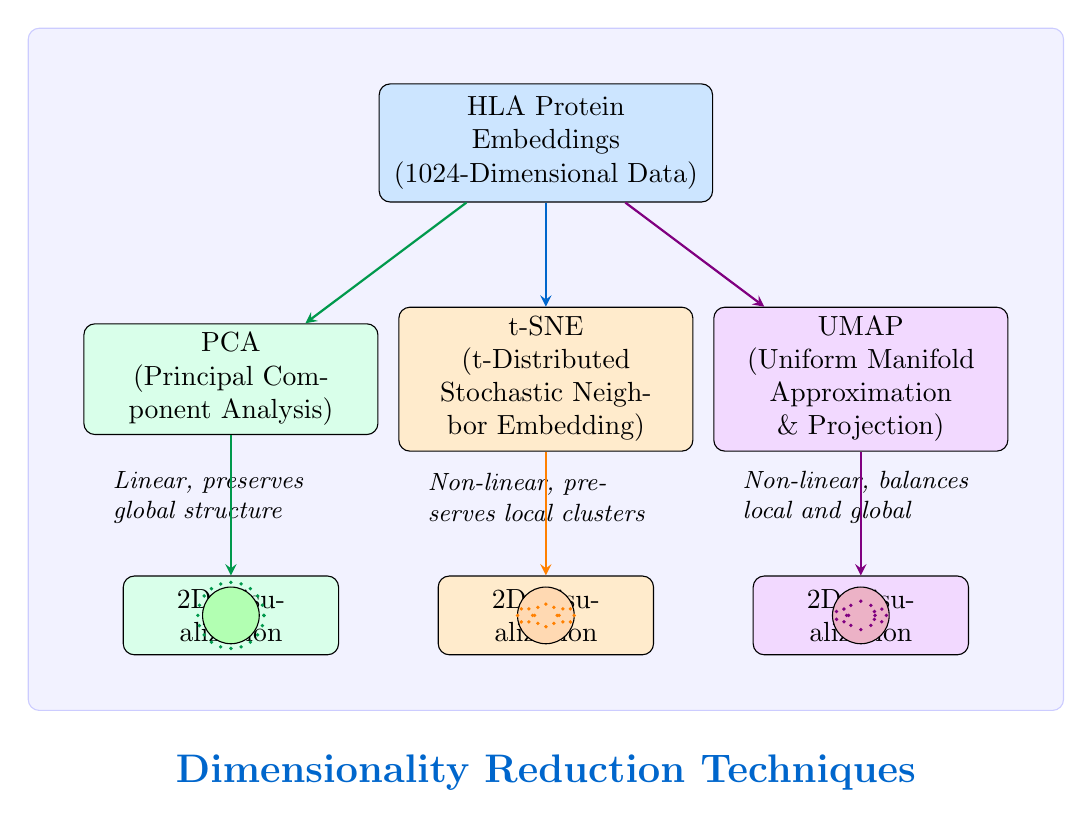
\begin{tikzpicture}[
    box/.style={draw, rounded corners, fill=white, text width=3.5cm, align=center, minimum height=1cm},
    arrow/.style={thick, ->, >=stealth},
    hidata/.style={draw, rounded corners, fill=hlalightblue, text width=4cm, align=center, minimum height=1.5cm},
    pca/.style={draw, rounded corners, fill=hlalightgreen, text width=3.5cm, align=center, minimum height=1cm},
    tsne/.style={draw, rounded corners, fill=hlalightorange, text width=3.5cm, align=center, minimum height=1cm},
    umap/.style={draw, rounded corners, fill=hlalightpurple, text width=3.5cm, align=center, minimum height=1cm},
    vis/.style={draw, rounded corners, text width=2.5cm, align=center, minimum height=1cm},
    note/.style={font=\small\itshape}
]

% High dimensional data
\node[hidata] (hidata) at (0,0) {HLA Protein Embeddings\\(1024-Dimensional Data)};

% Three dimensionality reduction techniques
\node[pca] (pca) at (-4,-3) {PCA\\(Principal Component Analysis)};
\node[tsne] (tsne) at (0,-3) {t-SNE\\(t-Distributed Stochastic Neighbor Embedding)};
\node[umap] (umap) at (4,-3) {UMAP\\(Uniform Manifold Approximation \& Projection)};

% Notes about each method
\node[note, text width=3cm, align=left] at (-4,-4.5) {Linear, preserves global structure};
\node[note, text width=3cm, align=left] at (0,-4.5) {Non-linear, preserves local clusters};
\node[note, text width=3cm, align=left] at (4,-4.5) {Non-linear, balances local and global};

% Visualizations
\node[vis, fill=hlalightgreen] (pcavis) at (-4,-6) {2D Visualization};
\node[vis, fill=hlalightorange] (tsnevis) at (0,-6) {2D Visualization};
\node[vis, fill=hlalightpurple] (umapvis) at (4,-6) {2D Visualization};

% Connect with arrows
\draw[arrow, hlablue] (hidata) -- node[right] {} (tsne);
\draw[arrow, hlagreen] (hidata) -- node[left] {} (pca);
\draw[arrow, hlapurple] (hidata) -- node[right] {} (umap);

\draw[arrow, hlagreen] (pca) -- (pcavis);
\draw[arrow, hlaorange] (tsne) -- (tsnevis);
\draw[arrow, hlapurple] (umap) -- (umapvis);

% Visualize each method with small example scatter plots
\begin{scope}[shift={(-4,-6)}, scale=0.12]
    % PCA visualization (more spread out, capturing variance)
    \filldraw[fill=green!30] (0,0) circle (3);
    \foreach \i in {0,...,20} {
        \pgfmathsetmacro{\x}{3.5*cos(18*\i)}
        \pgfmathsetmacro{\y}{3.5*sin(18*\i)}
        \fill[hlagreen] (\x,\y) circle (0.2);
    }
\end{scope}

\begin{scope}[shift={(0,-6)}, scale=0.12]
    % t-SNE visualization (tight clusters)
    \filldraw[fill=orange!30] (0,0) circle (3);
    \begin{scope}
        \foreach \i in {0,...,7} {
            \pgfmathsetmacro{\x}{1.2*cos(45*\i)}
            \pgfmathsetmacro{\y}{1.2*sin(45*\i)}
            \fill[hlaorange] (\x,\y) circle (0.2);
        }
    \end{scope}
    \begin{scope}[shift={(2.2,0)}]
        \foreach \i in {0,...,5} {
            \pgfmathsetmacro{\x}{0.8*cos(60*\i)}
            \pgfmathsetmacro{\y}{0.8*sin(60*\i)}
            \fill[hlaorange] (\x,\y) circle (0.2);
        }
    \end{scope}
    \begin{scope}[shift={(-2.2,0)}]
        \foreach \i in {0,...,5} {
            \pgfmathsetmacro{\x}{0.8*cos(60*\i)}
            \pgfmathsetmacro{\y}{0.8*sin(60*\i)}
            \fill[hlaorange] (\x,\y) circle (0.2);
        }
    \end{scope}
\end{scope}

\begin{scope}[shift={(4,-6)}, scale=0.12]
    % UMAP visualization (balance of clusters and structure)
    \filldraw[fill=purple!30] (0,0) circle (3);
    \begin{scope}
        \foreach \i in {0,...,7} {
            \pgfmathsetmacro{\x}{1.5*cos(45*\i)}
            \pgfmathsetmacro{\y}{1.5*sin(45*\i)}
            \fill[hlapurple] (\x,\y) circle (0.2);
        }
    \end{scope}
    \begin{scope}[shift={(2,0)}]
        \foreach \i in {0,...,4} {
            \pgfmathsetmacro{\x}{0.7*cos(72*\i)}
            \pgfmathsetmacro{\y}{0.7*sin(72*\i)}
            \fill[hlapurple] (\x,\y) circle (0.2);
        }
    \end{scope}
    \begin{scope}[shift={(-2,0)}]
        \foreach \i in {0,...,4} {
            \pgfmathsetmacro{\x}{0.7*cos(72*\i)}
            \pgfmathsetmacro{\y}{0.7*sin(72*\i)}
            \fill[hlapurple] (\x,\y) circle (0.2);
        }
    \end{scope}
\end{scope}

% Title
\node[align=center, font=\Large\bfseries, text=hlablue] at (0,-8) {Dimensionality Reduction Techniques};

% Background
\begin{scope}[on background layer]
    \node[fill=blue!5, draw=blue!20, rounded corners, inner sep=0.7cm, fit=(hidata) (pca) (tsne) (umap) (pcavis) (tsnevis) (umapvis)] {};
\end{scope}

\end{tikzpicture}
\end{document}
